\documentclass[margin=10pt]{standalone}
\usepackage{color,xcolor}
\usepackage{makecell}
\usepackage{tikz-qtree, tikz}
\usepackage[utf8]{inputenc}

\usetikzlibrary{spy,shapes.multipart,babel}
\usepackage[siunitx,europeanresistors,EFvoltages]{circuitikz} % To have the european convention for the drawing of electrical components. Also to have the current and voltage arrows going from high to low potential
\ctikzset{voltage/bump b=18pt,voltage/european label distance=15pt,voltage/distance from node=.1}
\definecolor{mygreen}{HTML}{258F1B}

\begin{document}
\renewcommand{\arraystretch}{1} % to increase the space between rows
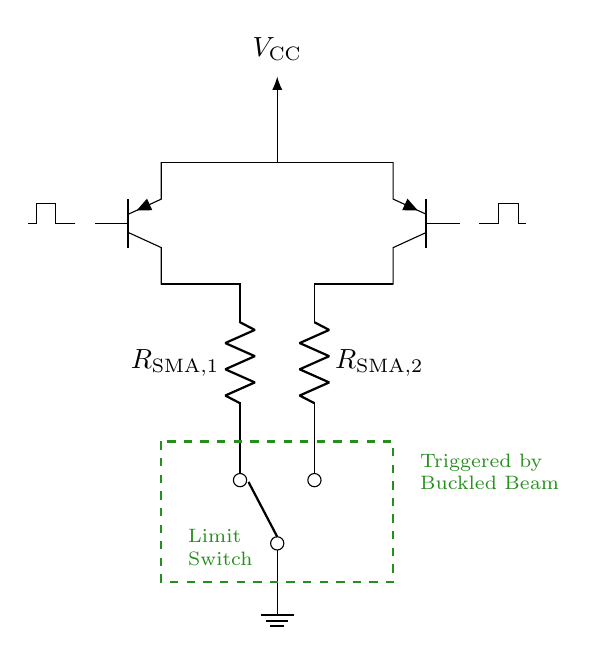
\begin{tikzpicture}[scale=1.0, transform shape]
    % \draw (-0.25,0) -- (0.25,0);
    \ctikzset{monopoles/vcc/arrow={Latex}}
    \draw (0,0) node[ground] (ground){}-- ++(0,0)node[spdt,anchor=in,scale=1.5,rotate=90] (Sw) {}
        (Sw.out 1) to[/tikz/circuitikz/bipoles/length=1.25cm,american resistor,l=$R_\mathrm{SMA,1}$] ++(0,2) coordinate(sma1top)-- ++(-1,0)node[pnp, anchor=C, xscale=1](pnp1){}
        (Sw.out 2) to[/tikz/circuitikz/bipoles/length=1.25cm,american resistor,l_=$R_\mathrm{SMA,2}$] ++(0,2) coordinate(sma2top)-- ++(1,0)node[pnp, anchor=C, xscale=-1](pnp2){}
        (pnp1.base) ++(-0.25,0)-- ++(-0.25,0)-- ++(0,0.25)-- ++(-0.25,0)-- ++(0,-0.25)-- ++(-0.1,0)
        (pnp2.base) ++(0.25,0)-- ++(0.25,0)-- ++(0,0.25)-- ++(0.25,0)-- ++(0,-0.25)-- ++(0.1,0)
        (pnp1.E) -| (0,6)
        (pnp2.E) -| (0,6)node[vcc,anchor=south]{$V_\mathrm{CC}$};

    \draw[dashed,mygreen,thick] let \p{Sw_i}=(Sw.in), \p{Sw_o1}=(Sw.out 1), \p{Sw_o2}=(Sw.out 2)  in (Sw.in)
    ($(\x{Sw_o1},\y{Sw_o1})+(-1,0)$) |- node[anchor=south west]{\scriptsize \begin{tabular}{l} Limit \\ Switch \end{tabular}} ($(\x{Sw_o2},\y{Sw_i})+(1,0)$) |- node[anchor=north west]{\scriptsize \begin{tabular}{l} Triggered by \\ Buckled Beam \end{tabular}} ($(\x{Sw_o1},\y{Sw_o1})+(-1,0)$);
\end{tikzpicture}
\renewcommand{\arraystretch}{1.5} % to increase the space between rows
\end{document}
